%%%%%%%%%%%%%%%%%%%%%%%%%%%%%%%%%%%%%%%%%
%
% (c) 2023 by Jennifer Laaser
%
% This work is licensed under the Creative Commons Attribution-NonCommercial-ShareAlike 4.0 International License. To view a copy of this license, visit http://creativecommons.org/licenses/by-nc-sa/4.0/ or send a letter to Creative Commons, PO Box 1866, Mountain View, CA 94042, USA.
%
% The current source for these materials is accessible on Github: https://github.com/jlaaser/pogil-polymers
%
%%%%%%%%%%%%%%%%%%%%%%%%%%%%%%%%%%%%%%%%%

\renewcommand{\figpath}{content/intro/nomenclature/figs}
\renewcommand{\labelbase}{nomenclature}

\begin{activity}{Polymer Nomenclature}

\begin{instructornotes}

	This activity introduces students to key concepts related to the nomenclature of polymers.
	
	After completing this activity, students will be able to:
			\begin{enumerate}
				\item \dots
			\end{enumerate}
			
	\subsection*{Activity summary:}
	\begin{itemize}
		\item \textbf{Activity type:} Learning Cycle
		\item \textbf{Content goals:} See above
		\item \textbf{Process goals:} %https://pogil.org/uploads/attachments/cj54b5yts006cklx4hh758htf-process-skills-official-pogil-list-2015-original.pdf
			\begin{itemize}
				\item Interpreting chemical structures
				\item Written and oral communication of reasoning
			\end{itemize}
		\item \textbf{Duration:} TBD
		\item \textbf{Instructor preparation required:} none beyond knowledge of relevant content
		\item \textbf{Related textbook chapters:}
			\begin{itemize}
				\item \emph{Polymer Chemistry} (Hiemenz \& Lodge), 2nd ed.: sections 1.3, 1.5, and 1.6
				\item \emph{Introduction to Polymres} (Young \& Lovell), 3rd ed.: section 1.2
			\end{itemize}
		%\item \textbf{Facilitation notes:}
		%	\begin{itemize}
		%		\item \dots
		%	\end{itemize}
	\end{itemize}

\end{instructornotes}

	%\textbf{Focus question:} Put a central question for the students to consider through this exercise here.

\begin{model}[Chain Chemistry]
\label{\labelbase:mdl:backsideend}

	When describing the chemistry of polymer chains, the three most important components of the molecule are the \emph{backbone}, the \emph{sidechains}, and the \emph{end groups}, as shown schematically below:
	
	\centerline{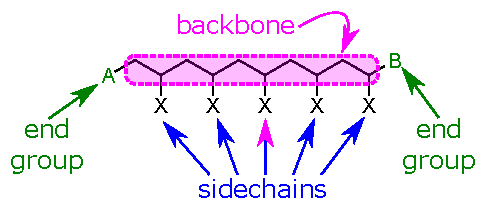
\includegraphics[width=0.5\textwidth]{\figpath/Model1_schematic.pdf}}

\end{model}


\begin{ctqs}

	\question Which of these components (backbone, sidechains, or end groups)...
	
		\begin{enumerate}
			\item ... contain the bonds and/or functional groups that make up the ``main chain'' that spans from one end of the polymer to the other?
			
				\begin{solution}[0.25in]
					backbone
				\end{solution}
			
			\item ... contain the functional groups that are attached to every repeat unit but are not part of unbroken string of bonds connecting one end of the polymer to the other?
			
				\begin{solution}[0.25in]
					sidechains
				\end{solution}
			
			\item ... ``cap'' the ends of the polymer chain?
			
				\begin{solution}[0.25in]
					end groups
				\end{solution}
				
		\end{enumerate}
		
	\question The structure of a polystyrene chain is given below:
	
		\centerline{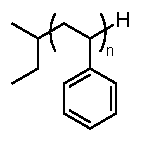
\includegraphics[width=0.15\textwidth]{\figpath/Model1_PS}}
	
		For this polymer, identify and sketch the structures of...
		\begin{enumerate}
			\item the backbone:
			
				\begin{solution}[0.75in]\studentdisplay{
					~
				}\instructordisplay{
					The backbone contains the string of C-C bonds highlighted below:
					
					\centerline{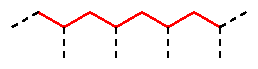
\includegraphics[width=0.3\textwidth]{\figpath/Model1_PS_backbone_soln}}
				}\end{solution}
			
			\item the sidechains:
			
				\begin{solution}[0.5in]\studentdisplay{
					~
				}\instructordisplay{
					The sidechains consist of the aromatic rings, as highlighted below:
					
					\centerline{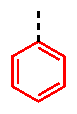
\includegraphics[width=0.075\textwidth]{\figpath/Model1_PS_sidechain_soln}}
				}\end{solution}
			
			\item the end groups:
			
				\begin{solution}[0.5in]\studentdisplay{
					~
				}\instructordisplay{
					The end groups are a sec-butyl group (left) and a hydrogen atom (right), as indicated below:
					
					\centerline{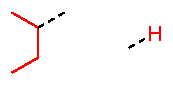
\includegraphics[width=0.2\textwidth]{\figpath/Model1_PS_endgrps_soln}}
				}\end{solution}
			
			
		\end{enumerate}
		
	\question Polystyrene is produced from the styrene monomer,
	
		\centerline{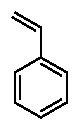
\includegraphics[width=0.1\textwidth]{\figpath/Model1_styrene}}
	
		\begin{enumerate}
			\item Upon polymerization, which bond from this monomer is incorporated into the backbone of the polymer chain?
			
				\begin{solution}[0.5in]
				
					The double bond is converted to a single bond and incorporated into the backbone of the chain.
					
				\end{solution}
				
			\item How is the structure of the repeat unit related to the structure of this monomer?
			
				\begin{solution}[0.5in]
				
					They have the same chemical formula and connectivity of the atoms, but the double bond in the monomer is replaced by a single bond in the polymer, and new bonds are formed to connect the monomer to the adjacent repeat units.
					
				\end{solution}
				
			\item How is the name of the polymer related to the name of this monomer?
			
				\begin{solution}[0.5in]
				
					The name of the polymer is just poly( name of the monomer ).
					
				\end{solution}
				
		\end{enumerate}
		
	\question Two other common polymers, and the monomers used to produce them, are shown below:
	
		\centerline{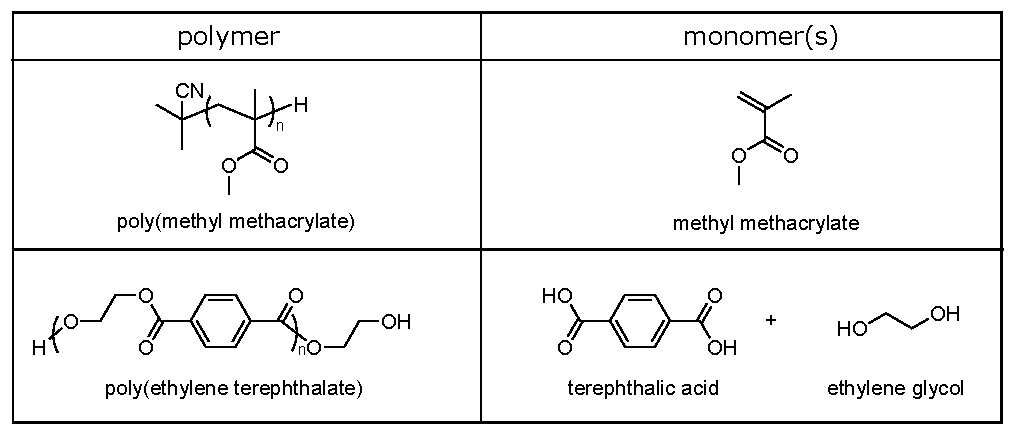
\includegraphics[width=0.8\textwidth]{\figpath/Model1_polymermonomertable}}
		
		Based on these structures, critique or defend each of the following statements in 2-3 complete sentences:
		
		\begin{enumerate}
			\item \emph{``Polymer chains always have backbones consisting of only C-C single bonds.''}
			
				\begin{solution}[1.5in]
					FALSE - clearly not true for PET!
				\end{solution}
			
			\item \emph{``Polymers are always named for the monomer from which they are produced.''}
			
				\begin{solution}[1.5in]
					FALSE - also clearly not true for PET!
				\end{solution}
			
		\end{enumerate}

\end{ctqs}

\begin{infobox}
	Polymers are typically named for their ``constituent repeat unit.''
\end{infobox}

\begin{ctqs}

	\question The structure of ethylene terephthalate is shown below:
	
		\centerline{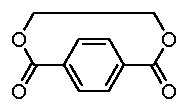
\includegraphics[width=0.2\textwidth]{\figpath/Model1_ethyleneterephthalate}}
		
		Is this structure consistent with the rule given in the above information box?  Briefly explain your group's reasoning.
		
		\begin{solution}[0.75in]
			Yes, it is.  This molecule has the same structure as the repeat unit of the poly(ethylene terephthalate) molecule, with only one bond needing to be broken/re-formed to link to adjacent repeat units.
			
			Note that IUPAC specifies clear rules for how the constituent repeat unit is named, which the above examples do not follow - we have given the ``common names'' for the repeat units rather than their IUPAC names.  See DOI 10.1351/PAC-REP-12-03-05 for a brief guide to IUPAC nomenclature.
		\end{solution}

\end{ctqs}


\clearpage


\begin{model}[Composition]
\label{\labelbase:mdl:composition}

	The polymers shown in Model \ref{\labelbase:mdl:backsideend} contain only one type of repeat unit.  However, it is also possible to produce polymers with multiple types of repeat units.  These polymers are usually classified in terms of how many distinct repeat units they contain, and how those repeat units are distributed throughout the chain.
	
	Several common classes of polymers are illustrated below:
	
	{\renewcommand{\arraystretch}{1.75}
	\begin{tabular}{m{0.78in}m{2in}m{2.5in}}
		\hline
		Classification & Repeat Unit Distribution & Example\\
		\hline
		Homopolymer & AAAAAAAAAAAAAAAAAA & 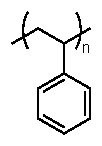
\includegraphics[width=0.4in]{\figpath/Model2_PS} ~~ poly(styrene) \\\hline
		Statistical Copolymer & ABBBABAABBAAAABBAB & 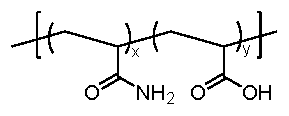
\includegraphics[width=1.25in]{\figpath/Model2_PAmAA} \newline poly(acrylamide-\emph{stat}-acrylic acid)\\\hline
		Alternating Copolymer & ABABABABABABABABAB & 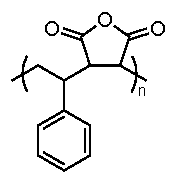
\includegraphics[width=0.75in]{\figpath/Model2_PSaltMA} \newline poly(styrene-\emph{alt}-maleic anhydride)\\\hline
		Diblock Copolymer & AAAAAAAAABBBBBBBBB & 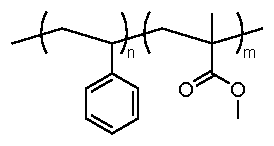
\includegraphics[width=1.25in]{\figpath/Model2_PSblockPMMA} \newline poly(styrene)-\emph{block}-poly(methyl methacrylate)\\\hline
		Triblock Copolymer & AAAAAABBBBBBAAAAAA & 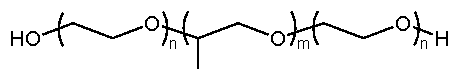
\includegraphics[width=2in]{\figpath/Model2_pluronic} \newline poly(ethylene oxide)-\emph{block}-poly(propyl\-ene oxide)-\emph{block}-poly(ethylene oxide) \\\hline
		Statistical Terpolymer & ABBCABACCCBCAABACB & 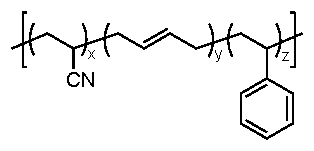
\includegraphics[width=1.5in]{\figpath/Model2_ABS} \newline poly(acrylonitrile-\emph{stat}-butadiene-\emph{stat}-styrene) \\\hline
		Graft Copolymer & 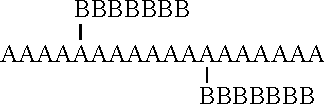
\includegraphics[width=1.75in]{\figpath/Model2_graftschematic} & 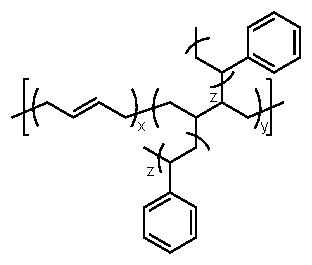
\includegraphics[width=1.25in]{\figpath/Model2_PBgPS} \newline poly(butadiene)-\emph{graft}-poly(styrene) 
	\end{tabular}
	}

\end{model}

\begin{ctqs}

	\question How many types of repeat units are included in...
	
		\begin{enumerate}
			\item ... homopolymers?
			
				\begin{solution}[0.25in]
				\end{solution}
			
			\item ... copolymers?
			
				\begin{solution}[0.25in]
				\end{solution}
			
			\item ... terpolymers?
			
				\begin{solution}[0.25in]
				\end{solution}
			
		\end{enumerate}
	
	\question For block copolymers, which part of the classification name indicates the number of polymer ``blocks''?
			
				\begin{solution}[0.5in]
				\end{solution}

	\question Compare the statistical, alternating, and diblock copolymers shown in the above table.
	
		\begin{enumerate}
		
			\item What are the key differences in how the repeat units are arranged in these three types of polymers?  Summarize your group's findings in 1-2 complete sentences.
			
				\begin{solution}[1.75in]
				\end{solution}
	
			\item How is the placement of the parentheses and/or brackets in the skeletal structures in the right-hand column used to indicate how the repeat units are arranged in these three types of polymers?  Summarize your group's findings in 1-2 complete sentences.
			
				\begin{solution}[1.75in]
				\end{solution}
			
		\end{enumerate}
		
	\question Using the rules you identified above, classify each of the following polymers: 
	
		(\emph{Challenge: if you have extra time, see if you can propose a formal name for each structure, too!})
	
		\begin{enumerate}
			\item \text{}\\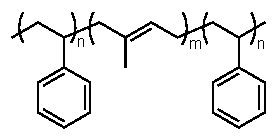
\includegraphics[width=0.25\textwidth]{\figpath/Model2_SBS}
			
				\begin{solution}[0.25in]
					triblock copolymer (poly(styrene)-\emph{block}-poly(butadiene)-\emph{block}-poly(styrene))
				\end{solution}
			
			\item \text{}\\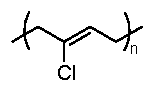
\includegraphics[width=0.15\textwidth]{\figpath/Model2_neoprene}
			
				\begin{solution}[0.25in]
					homopolymer (poly(chloroprene))
				\end{solution}
			
			\item \text{}\\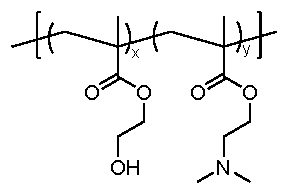
\includegraphics[width=0.25\textwidth]{\figpath/Model2_HEMAstatDMAEMA}
			
				\begin{solution}[0.25in]
					statistical copolymer (poly(hydroxyethyl methacrylate - \emph{stat} - dimethylaminoethyl methacrylate))
				\end{solution}
			
		\end{enumerate}
		
	\question Propose a possible sequence of a triblock terpolymer consisting of repeat units A, B, and C.
	
		\begin{solution}[0.5in]
		\end{solution}
	
	\question Draw the skeletal structure of a statistical copolymer of styrene and acrylonitrile.
	
		\begin{solution}[1in]
		\end{solution}
	
\end{ctqs}


\clearpage
\begin{model}[Isomerism]

	Even when polymers consist of only a single monomer, sometimes that monomer can be incorporated into the polymer chain in different ways.  This results in \textit{isomerism} in the polymer chain.  Three common types of isomerism are illustrated below:
	
	\begin{enumerate}
		\item Positional isomerism:
		
			\centerline{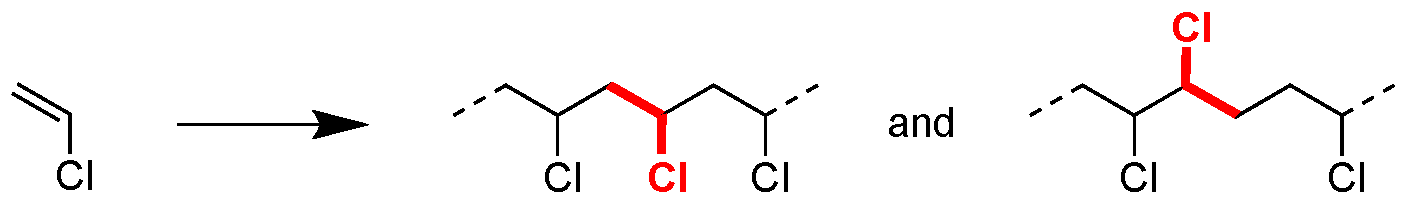
\includegraphics[width=0.8\textwidth]{\figpath/Model3_positional}}
		
		\item Stereoisomerism:
		
			\centerline{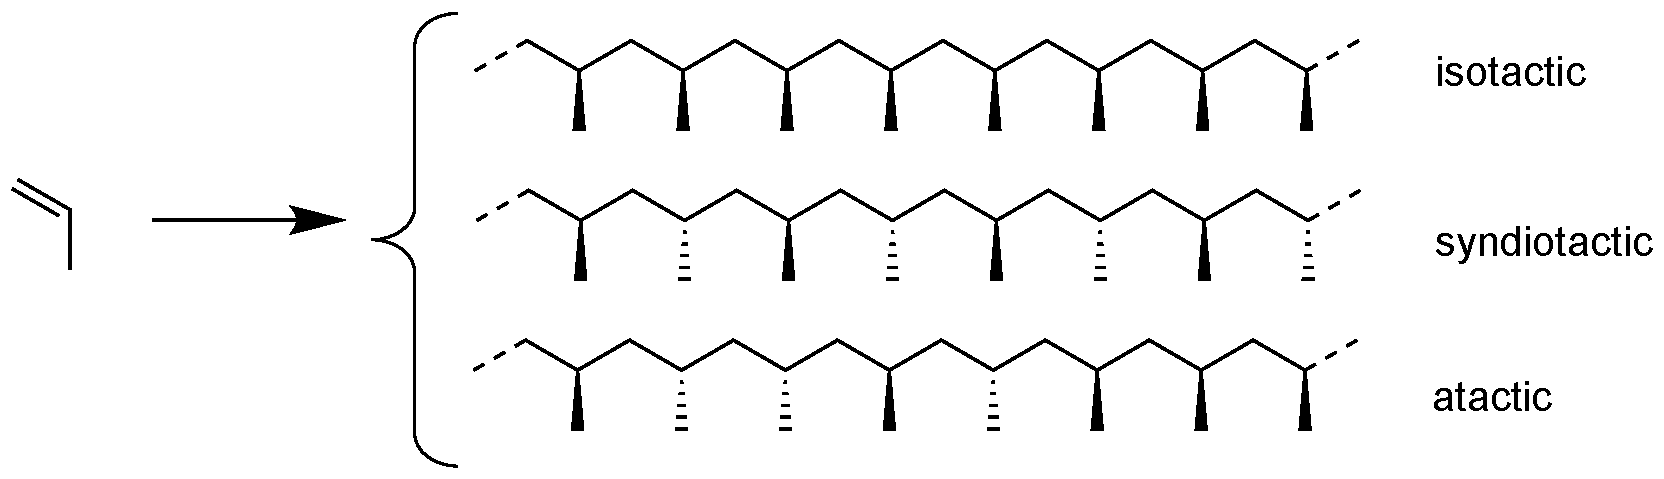
\includegraphics[width=0.8\textwidth]{\figpath/Model3_stereo}}
		
		\item Geometric isomerism:
		
		\vspace{4pt}	\centerline{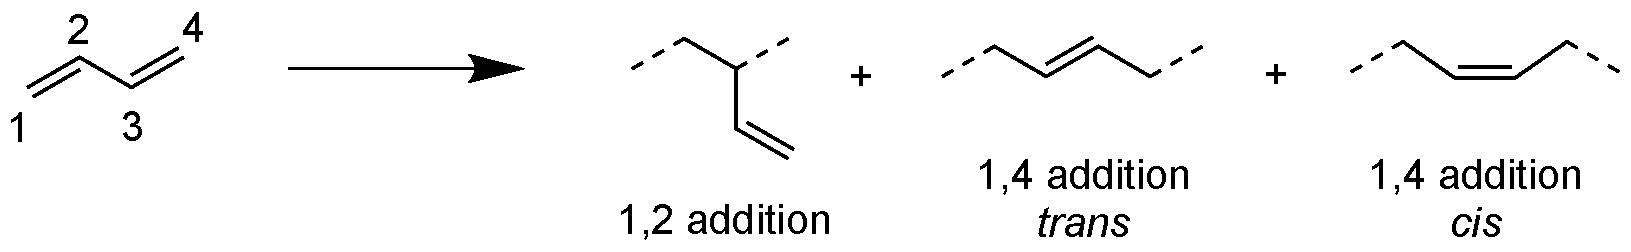
\includegraphics[width=0.8\textwidth]{\figpath/Model3_geometric}}
		
	\end{enumerate}

\end{model}

\begin{ctqs}

	\question What is the primary feature of the polymer chain that differs between...
	
		\begin{enumerate}
			\item ... different \emph{positional} isomers of the same monomer?
			
				\begin{solution}[0.5in]
				\end{solution}
			
			\item ... different \emph{stereoisomers} of the same monomer?
			
				\begin{solution}[0.5in]
				\end{solution}
			
			\item ... different \emph{geometric} isomers of the same monomer?
			
				\begin{solution}[0.5in]
				\end{solution}
			
		\end{enumerate}
		
	\question Sketch each of the following:
	
		\begin{enumerate}
			\item An 8 repeat-unit segment of syndiotactic poly(acrylonitrile):
			
				\begin{solution}[1in]
				\end{solution}
			
			\item The skeletal structure of a statistical copolymer of \emph{cis}-1,4 and \emph{trans}-1,4 polybutadiene:
			
				\begin{solution}[1in]
				\end{solution}
				
		\end{enumerate}
	
\end{ctqs}



\begin{exercises}

	%\exercise Poly(styrene) is an example of a ``vinyl-type'' polymer.  Vinyl-type polymers have the following general structure, as shown in Model \ref{\labelbase:mdl:backsideend}:
	
	%	IMAGE
		
	%	\begin{enumerate}
		
	%		\item Propose the structure of the monomer that is most likely used to produce this polymer.
			
	%			\emph{Hint: try replacing the aromatic ring in the structures shown in CTQs nnn and mmm with an ``X''!}
			
	%		\item Based on the structure you drew, explain, in 1-2 complete sentences, why these polymers are reasonably described as ``vinyl-type'' polymers.
			
	%	\end{enumerate}
		
	%\exercise Something about IUPAC nomenclature: 10.1351/PAC-REP-12-03-05
		
	%\exercise structure of kraton rubbers (SBS triblocks that then get hydrogenated?)
	
	%\exercise something about random vs statistical copolymers?
		
	\exercise The polymers shown in this activity were (almost) all \emph{linear} polymers, in which the backbone makes a single unbroken line from one end of the molecule to the other.  However, the backbone can also have more complex \emph{architectures}, some of which are illustrated below:
	
	\vspace{6pt}	\centerline{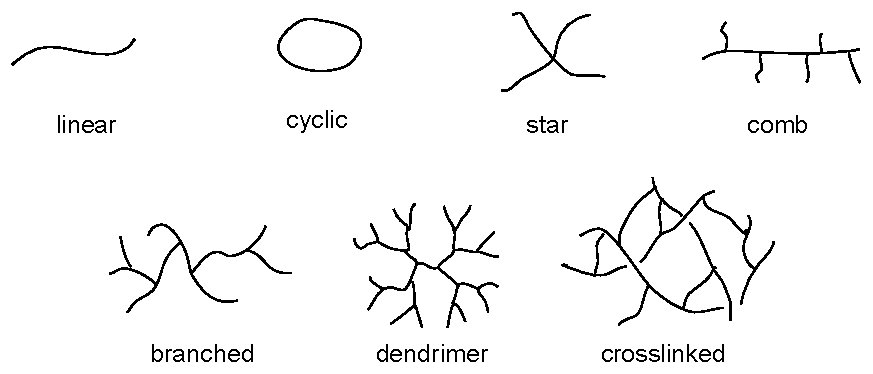
\includegraphics[width=0.7\textwidth]{\figpath/Exc_architectures}}
	
		Identify the architecture that most closely corresponds to each of the following chemical structures:
		
		\begin{enumerate}
			\item \text{}\\ 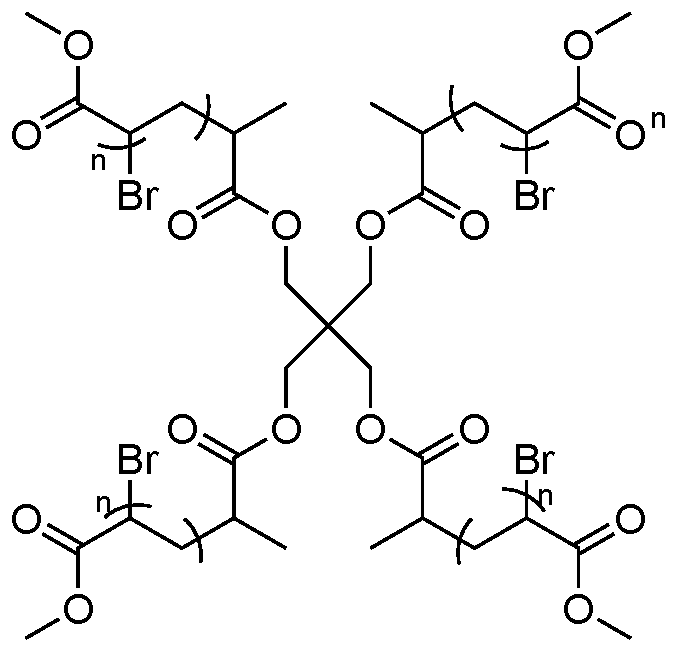
\includegraphics[width=0.3\textwidth]{\figpath/Exc_architectures_star}
			
			\item \text{}\\ 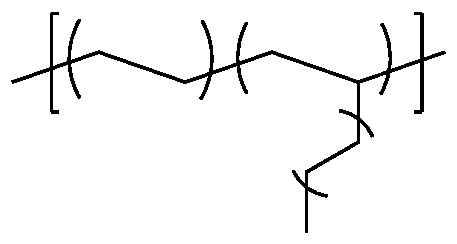
\includegraphics[width=0.2\textwidth]{\figpath/Exc_architectures_comb}
			
			\item \text{}\\ 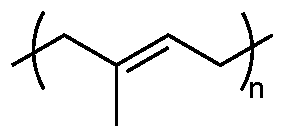
\includegraphics[width=0.15\textwidth]{\figpath/Exc_architectures_linear}
			
			\item \text{}\\ 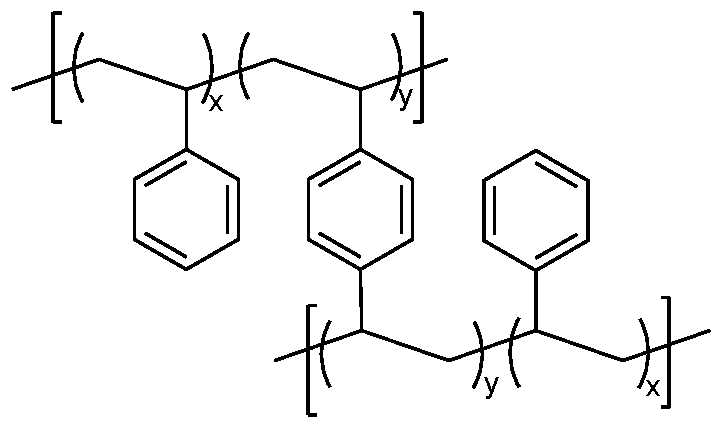
\includegraphics[width=0.3\textwidth]{\figpath/Exc_architectures_xlinked}
			
		\end{enumerate}
	
\end{exercises}

	
\end{activity}